\documentclass[12pt,journal,compsoc,draftcls]{IEEEtran}
\usepackage{listings}
\usepackage{cite}
\usepackage{graphicx}
\usepackage{float}
\usepackage[cmex10]{amsmath}
\usepackage{amsthm}
\usepackage{amsmath}
\usepackage{algorithmic}
\usepackage{program}
\usepackage{url}
\begin{document}

\title{Proving Correctness with Finite Automata}
\author{Jeremy Wright}
\markboth{CSE 355 Extra Credit Project with JFLAP Integration}
{Shell \MakeLowercase{\textit{et al.}}: Bare Demo of IEEEtran.cls for Computer Society Journals}

\IEEEcompsoctitleabstractindextext{%
\begin{abstract}
%\boldmath
Finite Automata recognize the class of regular languages. This class represents
the Type-3 grammars, the most restrictive, class from the Chomsky Hierarchy.
The beauty of this class is its simplicity. Simplicity allows us to prove
that the Finite Automata machines that recognize this class, generate the same
language. This permits one to prove that a program, represented by a FA,
completely, and solely implements a specification. Thereby proving correctness.
\end{abstract}

\begin{IEEEkeywords}
Deterministic Finite State Machine, Nondeterministic, Model Based Design
\end{IEEEkeywords}}
\maketitle


\IEEEdisplaynotcompsoctitleabstractindextext

\IEEEpeerreviewmaketitle

\section{Introduction}
\IEEEPARstart{P}{roving} a program is correct is the holy grail of software
engineering. Yet this illustrious goal is out of reach for some program domains.
A problem must be represented in a simple enough computational model in order to
prove its accuracy. The Chomsky Hierachy defines 4 grammar types of increasing
power \cite{wiki-chomsky}. This projects deals with the simplest of these
grammars, Type-3 regular-grammars.  These grammars form the basis for regular
expressions, and are described via finite automata. 

The class of regular languages has a powerful property. One can define a machine
that accepts 2 DFAs as in Equation \ref{eq:dfa}. From Sipser, we know that
Equation \ref{eq:dfa} is decidable \cite[p.~169]{Sipser}.
\begin{multline}
    EQ_{DFA} = \left\{ \langle A, B \rangle  \mid  L( A ) = L( B ) \right\} \\
    \text{Where A and B are DFAs}
    \label{eq:dfa}
\end{multline}
This forms the basis of our project. 

\hfill \today

\begin{figure*}[!t]
    \begin{center}
        \includegraphics[width=2.5in]{Correct.png}
        \label{fig:correct}
        \caption{Correct Implementation. Specification and Implementation are
        equal.}
    \end{center}
\end{figure*}

\begin{figure*}[!t]
    \centering
        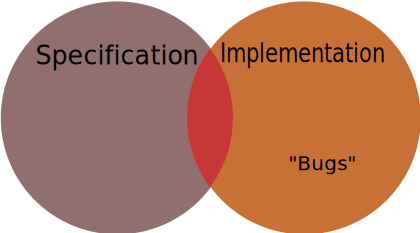
\includegraphics[width=2.5in]{BuggyImplementation.png}
        \label{fig:buggy}
        \caption{Buggy Implementation. ``Bugs'' are defined as strings part of
        the implementation which are not part of the specification.}
\end{figure*}
%\begin{figure*}[!t]
%    \begin{center}
%        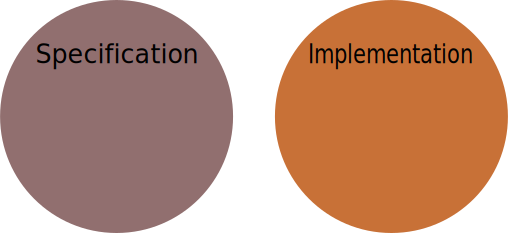
\includegraphics[width=2.5in]{disjoint.png}
%        \label{fig:disjoint}
%        \caption{Disjoint Implementation. Here the implementation implements no
%        part of the specification.}
%    \end{center}
%\end{figure*}
%\begin{figure*}[!t]
%    \begin{center}
%        \includegraphics[width=2.5in]{Scope-Creep.png}
%        \label{fig:scope-creep}
%        \caption{Referred to in industry as ``Scope-Creep'' the implementation
%        implements than is specified.}
%    \end{center}
%\end{figure*}
\begin{figure*}[!t]
    \begin{center}
        \includegraphics[width=2.5in]{IncompleteImplementation.png}
        \label{fig:incomplete}
        \caption{Incomplete Implementation. The specification describes
        a ``larger'' language than the implementation.}
    \end{center}
\end{figure*}

\section{Intuition}
Our goal is to build a system that can accept two ``programs'', one
a specification defining the correctness of the system. The second, an
implementation. Since the system leverages a property of regular languages the
problem must be simple enough to to express as a regular language i.e. the
problem must be expressable as a regular expression. 

Regular Languages are not extremely powerful, but some very useful tools,
such as grep, leverage Regular Languages. Another useful property of regular
languages is, regular languages are closed under the standard operations: union,
intersection, complement \cite[p.~45]{Sipser}.  We are now free to manipulate
our problem with standard set theory operations, and know we remain within the
context of regular languages.  

Our system will consume 2 programs, and our goal is to determine if your
specification matches our implementation as in Figure \ref{fig:correct}.
Equation \ref{eq:basis} defines how we intend to accomplish this. 
\begin{equation}
L( M ) = L( A ) \cup \overline{L ( S ) } 
\label{eq:basis}
\end{equation}

We simply then need to analyse L(M) to determine if our implementation matches
our specification. L(M) results 2 possiblities as equation \ref{eq:lmcases}
shows.
\begin{equation}
    L(M) = 
    \begin{cases}
        \emptyset \text{ if } L(A) \equiv L(S)\\
        \text{not empty if } L(A) \subset L(S) 
    \end{cases}
    \label{eq:lmcases}
\end{equation}

Intuitively this makes sense.  If a program has ``bugs'' then the language the
implementation describes is not fully contained by the implementation resuling
ins something akin to Figure \ref{fig:buggy}, furthermore its possible that the
implementation is fully contained by the specification, but the implementation
is still incomplete as in Figure \ref{fig:incomplete}.  Our Model checker simply
needs to accept 2 DFAs, and apply Equation \ref{eq:basis}.  If the result is an
empty language as in Equation \ref{eq:lmcases}, we know that the implementation
completely describes the specification.

\section{Model-Checker in C++}
The program design is composed of 


\subsection{Complexity}
Like, things get complex, and like some guy name Big-O comes and does something
about it. 
\appendices
\section{Quantum Computers and the Church-Turing Thesis}
\bibliographystyle{IEEEtran}
\bibliography{IEEEabrv,WrightSources}

\end{document}
